\documentclass[letter]{article}
\renewcommand{\baselinestretch}{1.25}

\usepackage[margin=1in]{geometry}
\usepackage{physics}
\usepackage{amsmath}
\usepackage{graphicx}
%\usepackage{pythonhighlight}
\usepackage{hyperref}
\usepackage{fancyvrb}

% MATLAB Formating Code
\usepackage[numbered,framed]{matlab-prettifier}
\lstset{style=Matlab-editor,columns=fullflexible}
\renewcommand{\lstlistingname}{Script}
\newcommand{\scriptname}{\lstlistingname}

% Command for easier minimization problem def
\newcommand{\optpblm}[3][eq:default]{
	\begin{equation}\label{#1}
% Array method... more centered		
%		\begin{array}{rl}
%			\text{minimize}  \hspace{0.2in} &#2 \vspace{5pt}\\
%			\text{subject to} \hspace{0.2in} &#3
%		\end{array}
% Aligned method... left aligned... idk if its better
		\begin{aligned}
			\text{minimize} \hspace{0.5in} &#2\vspace{5pt}\\
			\text{subject to \hspace{0.5in}} &#3
		\end{aligned}	
	\end{equation}
}

\allowdisplaybreaks

\title{MECH 6327 - Homework 3}
\author{Jonas Wagner}
\date{2021, March 24}

\begin{document}

\maketitle

\newpage
\tableofcontents

\newpage
\section*{BV Textobook Problems}
\subsection{Problem 4.11}
\textbf{Problem:}
Formulate each problem as a LP and explained the relationship between the optimal solution of the problems and the solution of its LP.\\
\textbf{Solution:}
\subsubsection{Part a: Minimize $\norm{Ax-b}_\infty$}
Define the following minimization problem:
\optpblm{\norm{Ax-b}_\infty}{\text{math}}
From the definition of an $\infty$-norm as $$\norm{x}_\infty = \max_i \abs{x_i}$$ the following can be derived:
\optpblm{t}{\qty(Ax - b)_i\leq t, \ \forall i = 1,\dots,n\\
		- & \qty(Ax - b)_i\leq t, \ \forall i = 1,\dots,n}
Which is equivalent to the following linear program
\optpblm{t}{-\vb{1}t \leq Ax - b \leq \vb{1}t}
The resulted minimum to this equivalent problem, $t*$, is equivalent to the minimum of the original problem, $\norm{Ax^*-b}_\infty$.

From this the minimizing variable, $x^*$, can be found as: $$x^* = A^{-1} (\vb{1}^T t^* + b)$$

\newpage
\subsubsection{Part b: Minimize $\norm{Ax-b}_1$}
Define the following minimization problem:
\optpblm{\norm{Ax-b}_1}{\text{math}}
From the definition of an $1$-norm as $$\norm{x}_1 = \sum_i \abs{x_i}$$ the following can be derived:
\optpblm{t_1 + \cdots + t_n}{\qty(Ax - b)_i\leq t_i, \ \forall i = 1,\dots,n\\
-	& \qty(Ax - b)_i\leq t_i, \ \forall i = 1,\dots,n}
Which is equivalent to the following linear program
\optpblm{\vb{1}^T t}{-t \leq Ax - b \leq t}
The resulted minimum to this equivalent problem, $\vb{1}^T t$, is equivalent to the minimum of the original problem, $\norm{Ax-b}_1$.

From this the minimizing variable, $x^*$, can be found as: $$x^* = A^{-1} (t^* + b)$$

\newpage
\subsubsection{Part c: Minimize $\norm{Ax-b}_1$ subject to $\norm{x}_{\infty}\leq 1$}
Define the following minimization problem:
\optpblm{\norm{Ax-b}_1}{\norm{x}_\infty \leq 1}
From the definition of an $1$-norm as $$\norm{x}_1 = \sum_i \abs{x_i}$$ and the definition of an $\infty$-norm as $$\norm{x}_\infty = \max_i \abs{x_i}$$ the following can be derived:
\optpblm{t_1 + \cdots + t_n}{\qty(Ax - b)_i\leq t_i, \ \forall i = 1,\dots,n\\
	-& \qty(Ax - b)_i\leq t_i, \ \forall i = 1,\dots,n\\
	 & x_i \leq 1, \forall i = 1,\dots,n\\
	-& x_i \leq 1, \forall i = 1,\dots,n}
Which is equivalent to the following linear program
\optpblm{\vb{1}^T t}{-t \leq Ax - b \leq t\\
					&-\vb{1} \leq x \leq \vb{1}}

The resulted minimum to this equivalent problem, $\vb{1}^T t$, is equivalent to the minimum of the original problem, $\norm{Ax-b}_1$.

From this the minimizing variable, $x^*$, can be found as: $$x^* = A^{-1} (t^* + b)$$

\newpage
\subsubsection{Part d: Minimize $\norm{x}_1$ subject to $\norm{Ax-b}_\infty \leq 1$}
Define the following minimization problem:
\optpblm{\norm{x}_1}{\norm{Ax-b}_\infty \leq 1}
From the definition of an $1$-norm as $$\norm{x}_1 = \sum_i \abs{x_i}$$ and the definition of an $\infty$-norm as $$\norm{x}_\infty = \max_i \abs{x_i}$$ the following can be derived:
\optpblm{t_1 + \cdots + t_n}{x_i \leq t_i, \ \forall i = 1,\dots,n\\
							&-x_i \leq t_i, \ \forall i = 1,\dots,n\\
							&(Ax-b)_i \leq 1, \ \forall i = 1,\dots,n}
From this a linear program can be defined as:
\optpblm{\vb{1}^T t}{-t \leq x \leq t\\
			 		&Ax - b \leq \vb{1}}

The resulted minimum to this equivalent problem, $\vb{1}^T t$, is equivalent to the minimum of the original problem, $\norm{x}_1$.

From this the minimizing variable, $x^*$, can be found as: $$x^* = t^*$$

\newpage
\subsubsection{Part e: Minimize $\norm{Ax-b}_1 + \norm{x}_\infty$}
Define the following minimization problem:
\optpblm{\norm{Ax-b}_1 + \norm{x}_\infty}{math}
From the definition of an $1$-norm as $$\norm{x}_1 = \sum_i \abs{x_i}$$ and the definition of an $\infty$-norm as $$\norm{x}_\infty = \max_i \abs{x_i}$$ the following can be derived:
\optpblm{t_1 + \cdots + t_n + s}{
		\qty(Ax - b)_i\leq t_i, \ \forall i = 1,\dots,n\\
		-& \qty(Ax - b)_i\leq t_i, \ \forall i = 1,\dots,n\\
		&x_i \leq s, \ \forall i = 1,\dots,n\\
	-	&x_i \leq s, \ \forall i = 1,\dots,n}
This can be written as a standard linear program as:
\optpblm{\vb{1}^T t + s}{
		- t \leq Ax-b \leq t\\
		&-\vb{1}s \leq x \leq \vb{1}s}
The resulted minimum to this equivalent problem, $\vb{1}^T t + s$, is equivalent to the minimum of the original problem, $\norm{Ax-b}_1 + \norm{x}_\infty$. It should be noted that the $s$ and $\norm{x}_\infty$ are not used to find the minimization variable, but are important in weighting for solving for the minimization itself.

From this the minimizing variable, $x^*$, can be found as: $$x^* = A^{-1} (t^* + b)$$

\newpage
\subsection{Problem 4.16}
Consider the system given as
\begin{equation}\label{eq:dyn_sys_def}
	x(t+1) = A x(t) + b u(t), \ t = 0,\dots,N-1
\end{equation}
with $x(t) \in \real^n, u(t) \in \real, \forall t = 0,\dots,N-1$ and $A \in \real^{n\cross n}, b \in \real^n$, and $x(0) = 0$.\\

The minimum fuel optimal control problem is to select the minimum amount of inputs to minimize the amount of fuel used, given as
\begin{equation}\label{eq:min_fuel_problem_def}
	\begin{aligned}
		\text{minimize} \hspace{0.5in} &F = \sum_{t=1}^{N-1} f(u(t))\\
		\text{subject to \hspace{0.5in}} & x(t+1) = A x(t) + b u(t), \ t = 0,\dots,N-1\\
		& x(N) = x_{des}
	\end{aligned}	
\end{equation}
with $N$ as the time-horizon, $x_{des} \in \real^n$ as the desired final state, and $f: \real \to \real$ given as
\begin{equation}\label{eq:fuel_usage_def}
	f(a) = 
	\begin{cases}
		\abs{a} & \abs{a} \leq 1 \\
		2 \abs{a} - 1 & \abs{a} > 1
	\end{cases}
\end{equation}

\textbf{Problem:}
Formulate this problem as a Linear Program.\\

\textbf{Solution:}
First, \ref{eq:min_fuel_problem_def} can be rewritten in an epigraph form (with the additional assumption that $f(u(t))$ is always positive):
\optpblm[eq:min_fuel_problem_epigraph]{F_1 + \cdots + F_{N-1}}{
		f(u(t)) = F_t, \ \forall t = 1, \dots, N-1\\
		& x(t+1) = A x(t) + b u(t), \ \forall t = 0,\dots,N-1\\
		&x(N) = x_{des}}
Now looking at the nonlinear component, fuel usage as defined by \eqref{eq:fuel_usage_def}, can be equated to:
\begin{equation}
	\begin{aligned}
		\abs{a} \leq g\\
		2 \abs{a} - 1 \leq g\\
	\end{aligned}
\end{equation}
or equivalently,
\begin{equation}
	\begin{aligned}
		-g \leq a \leq g\\
		-g \leq 2a -1 \leq g
	\end{aligned}
\end{equation}

This represents an intersection of two half-spaces which is a simpliler convex restriction.\\
This can now be combined with \eqref{eq:min_fuel_problem_epigraph} to produce the linear program:
\optpblm[eq:min_fuel_problem_result]{F_1 + \cdots + F_{N-1}}{
	-F_t \leq u(t) \leq F_t, \ \forall t = 1, \dots, N-1\\
	&-F_t \leq 2u(t) -1 \leq F_t, \ \forall t = 1, \dots, N-1\\
	& x(t+1) = A x(t) + b u(t), \ \forall t = 0,\dots,N-1\\
	&x(N) = x_{des}}
Which can then be rewritten as:
\optpblm[eq:min_fuel_problem_result]{\vb{1}^T F}{
	-F \leq \vb{u} \leq F\\
	& x(t+1) = A x(t) + b u(t), \ \forall t = 0,\dots,N-1\\
	&x(N) = x_{des}
	}

\newpage
\subsection{Problem 4.28}
Consider the convex quadratic program given as
\begin{equation}\label{eq:convex_quadratic_program}
	\begin{aligned}
		\text{minimize} \ \ & \frac{1}{2} x^T P x + q^T x + r\\
		\text{subject to} \ \ & Ax \leq b
	\end{aligned}
\end{equation}
with a robust equivalent defined as
\begin{equation}\label{eq:robust_convex_quadratic_program}
	\begin{aligned}
		\text{minimize} \ \ & \sup_{P\in \mathcal{E}}\{\frac{1}{2} x^T P x + q^T x + r\}\\
		\text{subject to} \ \ & Ax \leq b
	\end{aligned}
\end{equation}
where $\mathcal{E}$ is the set of all possible matrices of $P$.

\subsubsection{Part a}
\textbf{Problem:}
Express the robust QP as a convex problem given $\mathcal{E} = \{P_1,\dots,P_k\}$ where $P_i\in S^n_+, \ \forall i=1,\dots,k$.\\

\textbf{Solution:}
As a base assumption, by definition all quadratic programs are convex. Additionally when taking a pointwise supremum of convex sets, the result is also convex.
Thus, for a supremum over the finite set of $\mathcal{E}$ it is known that a resultant convex problem can be defined.\\

First, we can redefine the problem as
\optpblm{\sup \{t_1, \dots, t_k\}}{
	\frac{1}{2} x^T P_i x + q^T x + r \leq t_i, \ i = 1, \dots, k\\
	&Ax \leq b}
Another eipigraph can then be analyzed to create the following convex optimization problem:
\optpblm{s}{
	t_i \leq s, \ i = 1, \dots, k\\
	&\frac{1}{2} x^T P_i x + q^T x + r \leq t_i, \ i = 1, \dots, k\\
	&Ax \leq b}


% no part b,c for 4.28


\newpage
\subsection{Problem 4.43}
Suppose $A: \real^n \to S^m$ is affine such that
\begin{equation}
	A(x) = A_0 + x_1 A_1 + \cdots + x_n A_n
\end{equation}
where $A_i \in S^m$. Let $\lambda_1(x) \geq \lambda_2(x) \geq \cdots \geq \lambda_m(x)$ be the eigenvalues of $A(x)$.\\


For each of the following minimization criteria, formulate the problem as an SDP.\\

\subsubsection{Part a}
\textbf{Problem:}
Minimize the maximum eigenvalue of $A$: $$\text{minimize} \ \ \lambda_1(x)$$
\textbf{Solution:}
This ca be re-written in epigraph form as:
\optpblm{t}{\lambda_1 \leq t}
or similarily as an SDP:
\optpblm{t}{A(x) \preceq t I}


%It is known that the eigenvalues of a sum of matrices is bounded below by the sum of the minimum eigenvalues of each and bounded above by the sum of the maximum eigenvalues.
%\cite{eigvalueBound}
%i.e.
%$$ \lambda(A)_m + \lambda(B)_m \leq \lambda(A+B)_m \leq \lambda(A+B)_1 \leq \lambda(A)_1 + \lambda(B)_1$$
%If this is to be expanded to the entire affine sum, $A(x)$, the objective of minimizing the eigenvalues of the weighted sum of symetric matrices can be done by minimizing the weighted sum of the largest eigenvalues of individual matrices.
%This means this problem can be redefined as:
%\optpblm{t^T x}{
%	t_i = \lambda_1(A_i), \ \forall i = 1,\dots,m\\
%	&s = \lambda_1(A_0)}
%Since $s$ will remain constant regrdless of $x$, this is equivalent to:
%\optpblm{t^T x}{
%	t_i = \lambda_1(A_i), \ \forall i = 1,\dots,m}
%
%????????????????????????????????????????????????????

\subsubsection{Part b}
\textbf{Problem:}
Minimize the spread of the eigenvalues of $A$: $$\text{minimize} \ \ \lambda_1(x) - \lambda_m(x)$$\\
\textbf{Solution:}
This can be rewritten in epigraph form as
\optpblm{t_1 - t_2}{\lambda_1 \leq t_1\\ & \lambda_m \leq t_2}
or similarly as an SDP:
\optpblm{t_1}{A(x) \preceq t_1 I\\ &A(x) \succeq t_2}


%It is known that the eigenvalues of a sum of matrices is bounded below by the sum of the minimum eigenvalues of each and bounded above by the sum of the maximum eigenvalues.
%\cite{eigvalueBound}
%i.e.
%$$ \lambda(A)_m + \lambda(B)_m \leq \lambda(A+B)_m \leq \lambda(A+B)_1 \leq \lambda(A)_1 + \lambda(B)_1$$
%If this is to be expanded to the entire affine sum, $A(x)$, the objective of minimizing the spread eigenvalues of the weighted sum of symetric matrices can be done by minimizing the weighted sum of the spread of eigenvalues of individual matrices.
%This means this problem can be redefined as:
%\optpblm{t^T x + s}{
%	t_i = (\lambda_1(A_i) - \lambda_m(A_i), \ \forall i = 1,\dots,m\\
%	&s = (\lambda_1(A_0) - \lambda_m(A_0)}
%Since $s$ remains constant regardless of $x$ this is equivelent to
%\optpblm{t^T x}{
%	t_i = (\lambda_1(A_i) - \lambda_m(A_i), \ \forall i = 1,\dots,m}
%
%
%????????????????????????????????????????????????????


%Defining the optimization problem as:
%\optpblm{\max \{\lambda\qty(A(x))\} - \min \{\lambda\qty(A(x))\}}{
%	A(x) = A_0 + x_1 A_1 + \cdots + x_n A_n}\\


%
%WHAT???

\newpage
\subsubsection{Part c}
\textbf{Problem:}
Minimize the conditional number of $A$ while remaining postive definite:
\begin{equation*}
	\begin{aligned}
		\text{minimize} \ \ &k(A(x)) = \frac{\lambda_1(x)}{\lambda_m(x)} \ \forall \ x \in \{x \ | \ A(x) \succ 0\}\\
		 \text{subject to} \ \ &A(x) \succ 0
	\end{aligned}
\end{equation*}
\textbf{Solution:}
This can be rewritten in epigraph form as
\optpblm{t_1 / t_2}{
	\lambda_1 \leq t_1\\
	& \lambda_m \leq t_2\\
	&A \succ 0
	}
or similarly as an SDP:
\optpblm{t_1 / t_2}{
	A(x) \preceq t_1 I\\
	&A(x) \succeq t_2\\
	&A \succ 0
	}

% Only Part a,b,c for 4.43

\newpage
\section{Problem 1: Open-loop optimal control with $1-$ and $\infty-$ norms.}
The following open-loop optimal regulation problem is given as:
\begin{equation}\label{eq:open-loop_opt-control_def}
	\begin{aligned}
		\text{minimze} \hspace{0.5in}
		&\norm{x_T}_p + \sum_{t = 0}^{T-1} \norm{x_t}_p + \gamma\norm{u_t}_q\\
		\text{subject to} \hspace{0.5in}
		& x_{t+1} = A x_t + B u_t, \ t = 0,\dots,T-1\\
		& \norm{x_t}_\infty \leq \bar{x}, \ t = 0,\dots,T\\
		& \norm{u_t}_\infty \leq \bar{u}, \ t = 0,\dots,T
	\end{aligned}
\end{equation}
with $x_t \in \real^n$ and $u_t \in \real^m$ as the system state and control input respectively and parameter $\gamma > 0$ governing the actuator and state regulation performance.\\

\textbf{Problem:}
Express this problem as a linear program for (i) $p=q=\infty$ and (ii) $p=q=1$. Code both in CVX and for the problem data provided. Verify the equivalence between the original optimization problem and transformed linear program obtained and plot the optimal state and input trajectories for each.\\

\textbf{Solution:}
\subsection{Linear program for $p = q = \infty$}

With $p = q = \infty$, the problem is defined as:
\optpblm{\norm{x_T}_\infty + \sum_{t = 0}^{T-1} \norm{x_t}_\infty + \gamma\norm{u_t}_\infty}{
	x_{t+1} = A x_t + B u_t, \ t = 0,\dots,T-1\\
	& \norm{x_t}_\infty \leq \bar{x}, \ t = 0,\dots,T\\
	& \norm{u_t}_\infty \leq \bar{u}, \ t = 0,\dots,T}

The epigraph of this problem can be found as
\optpblm{r_T + (r_0 + \gamma s_0) + (r_{T-1} + \gamma s_{T-1})}{
	\norm{x_t}_\infty \leq r_t, \ t = 0, \dots, T\\
	&\norm{u_i}_\infty \leq s_t, \ t = 0, \dots, T-1\\
	&x_{t+1} = A x_t + B u_t, \ t = 0,\dots,T-1\\
	& \norm{x_t}_\infty \leq \bar{x}, \ t = 0,\dots,T\\
	& \norm{u_t}_\infty \leq \bar{u}, \ t = 0,\dots,T
	}

From the definition of $\norm{x}_\infty = \max \{x\}$ and through vectorization, we can redefine this as the following linear program:
\optpblm{
	\mqty[\vb{1}^T & \gamma \vb{1}^T] \mqty[r\\s] 
	=\vb{1}^T r + \gamma \vb{1}^T s}{
	x_{t+1} = A x_t + B u_t, \ t = 0,\dots,T-1\\
	&x_t \leq r_t \vb{1} \leq \bar{x} \vb{1}, \ t = 0, \dots, T\\
	&u_t \leq s_t \vb{1} \leq \bar{u} \vb{1}, \ t = 0, \dots, T-1
	}

\subsection{Linear program for $p = q = 1$}
With $p = q = 1$, the problem is defined as:
\optpblm{\norm{x_T}_1 + \sum_{t = 0}^{T-1} \norm{x_t}_1 + \gamma\norm{u_t}_1}{
	x_{t+1} = A x_t + B u_t, \ t = 0,\dots,T-1\\
	& \norm{x_t}_\infty \leq \bar{x}, \ t = 0,\dots,T\\
	& \norm{u_t}_\infty \leq \bar{u}, \ t = 0,\dots,T}

The epigraph of this problem can be found as
\optpblm{r_T + (r_0 + \gamma s_0) + (r_{T-1} + \gamma s_{T-1})}{
	\norm{x_t}_1 \leq r_t, \ t = 0, \dots, T\\
	&\norm{u_i}_1 \leq s_t, \ t = 0, \dots, T-1\\
	&x_{t+1} = A x_t + B u_t, \ t = 0,\dots,T-1\\
	& \norm{x_t}_\infty \leq \bar{x}, \ t = 0,\dots,T\\
	& \norm{u_t}_\infty \leq \bar{u}, \ t = 0,\dots,T
}

From the definition of $\norm{x}_1 = \sum_{i=0}^T x$ and through vectorization, we can redefine this as the following linear program:
\optpblm{
	\mqty[\vb{1}^T & \gamma \vb{1}^T] \mqty[r\\s] 
	=\vb{1}^T r + \gamma \vb{1}^T s}{
	x_{t+1} = A x_t + B u_t, \ t = 0,\dots,T-1\\
	& \vb{1}^T x_t \leq r_t, \ t = 0,\dots,T\\
	& \vb{1}^T u_t \leq s_t, \ t = 0,\dots,T-1\\
	&x_t \leq \bar{x} \vb{1}, \ t = 0, \dots, T\\
	&u_t \leq \bar{u} \vb{1}, \ t = 0, \dots, T-1
}


\newpage
\subsection{CVX Formulation and Results:}
The code used to solve the linear programs and direct norm cvx calculations can be found in \appendixname \ref{apx:pblm1_matlab}.\\

\subsubsection{$\infty$-norm Solution}
\begin{figure}[h]
	\centering
	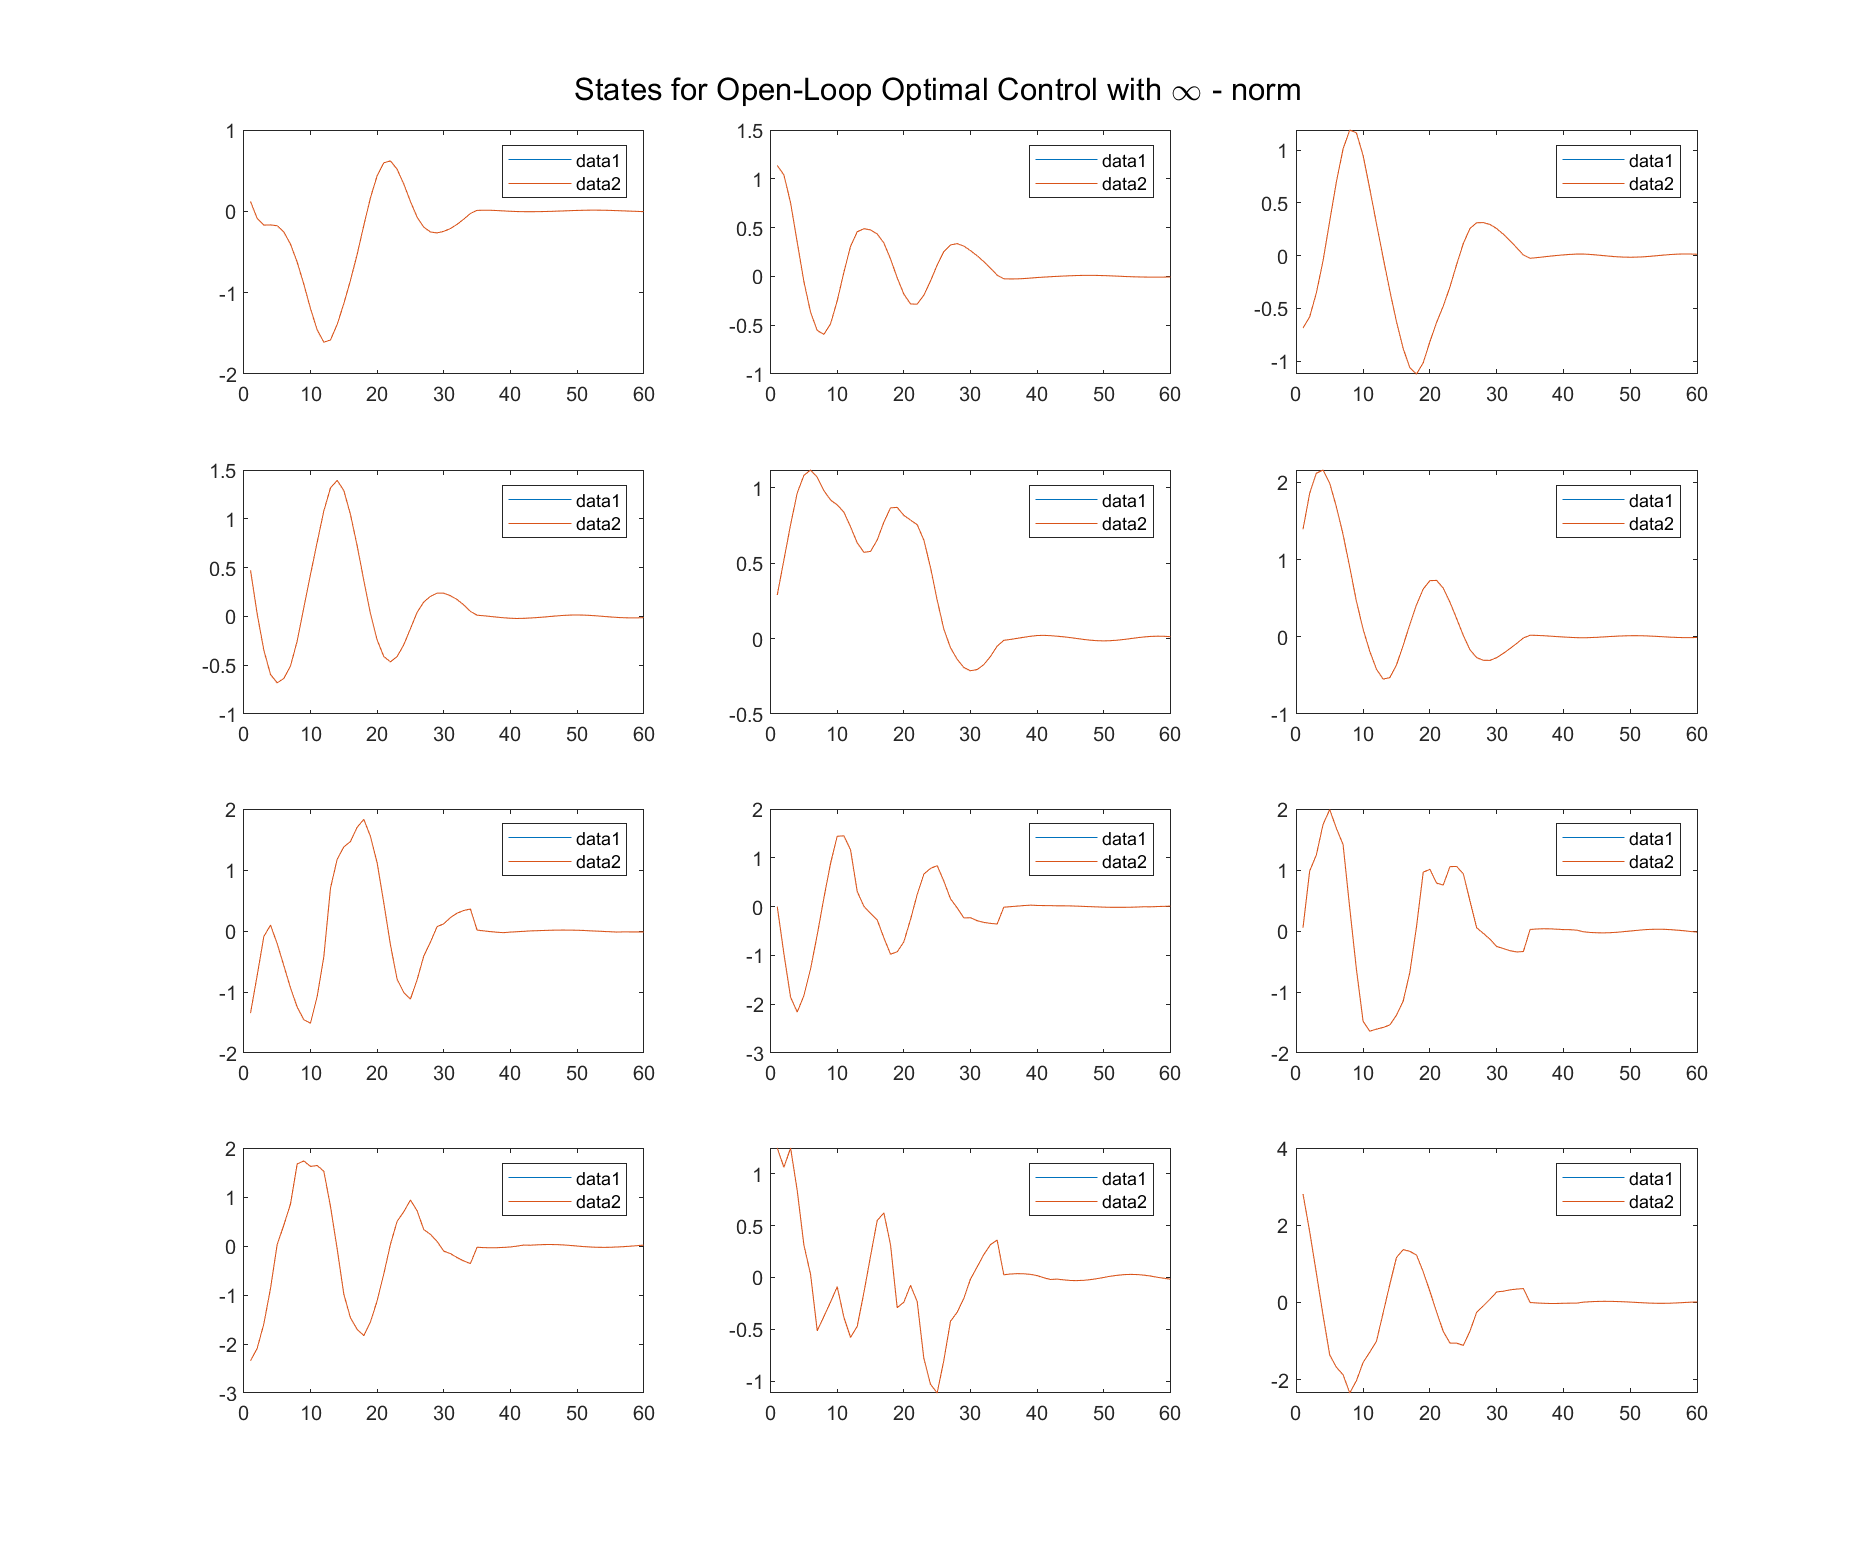
\includegraphics[width=1\linewidth]{fig/pblm1_inftyn_x}
	\caption{States for Open-loop control comparing methods for $\infty$-norm.}
	\label{fig:pblm1inftynx}
\end{figure}\newpage

\begin{figure}[h]
	\centering
	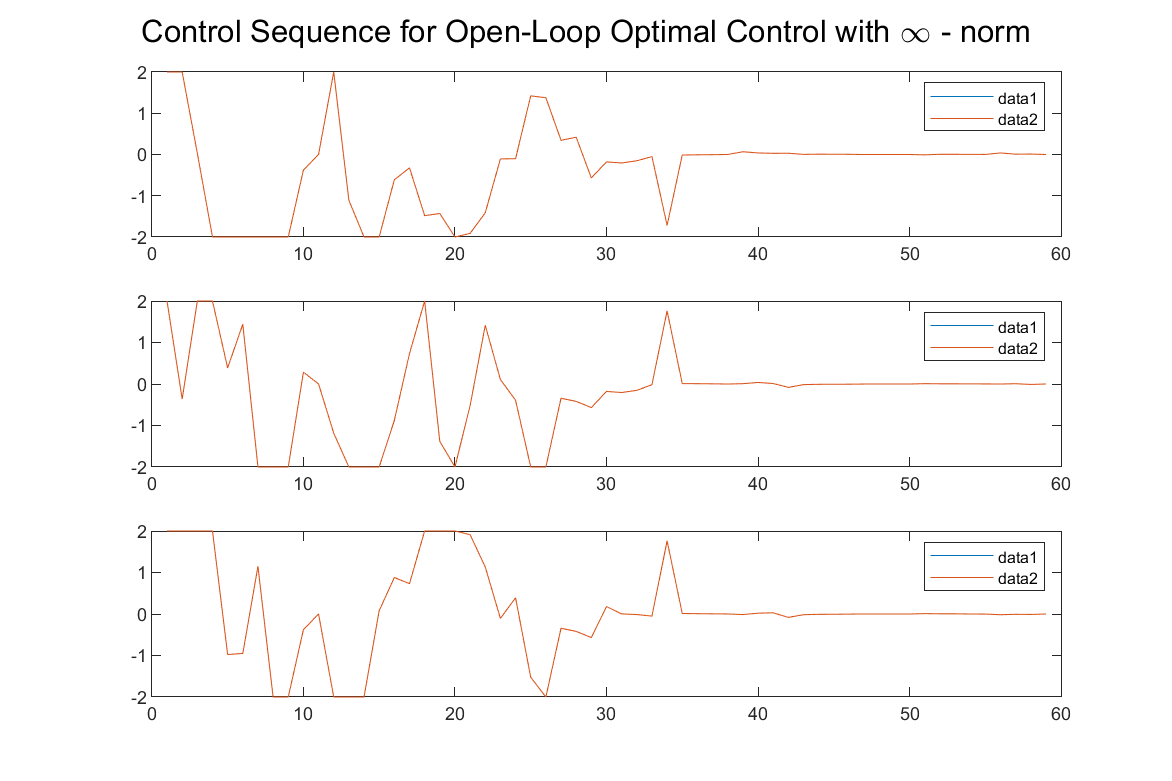
\includegraphics[width=1\linewidth]{fig/pblm1_inftyn_u}
	\caption{Inputs for Open-loop control comparing methods for $\infty$-norm.}
	\label{fig:pblm1inftynu}
\end{figure}\newpage

\subsubsection{1-norm Solution}
\begin{figure}[h]
	\centering
	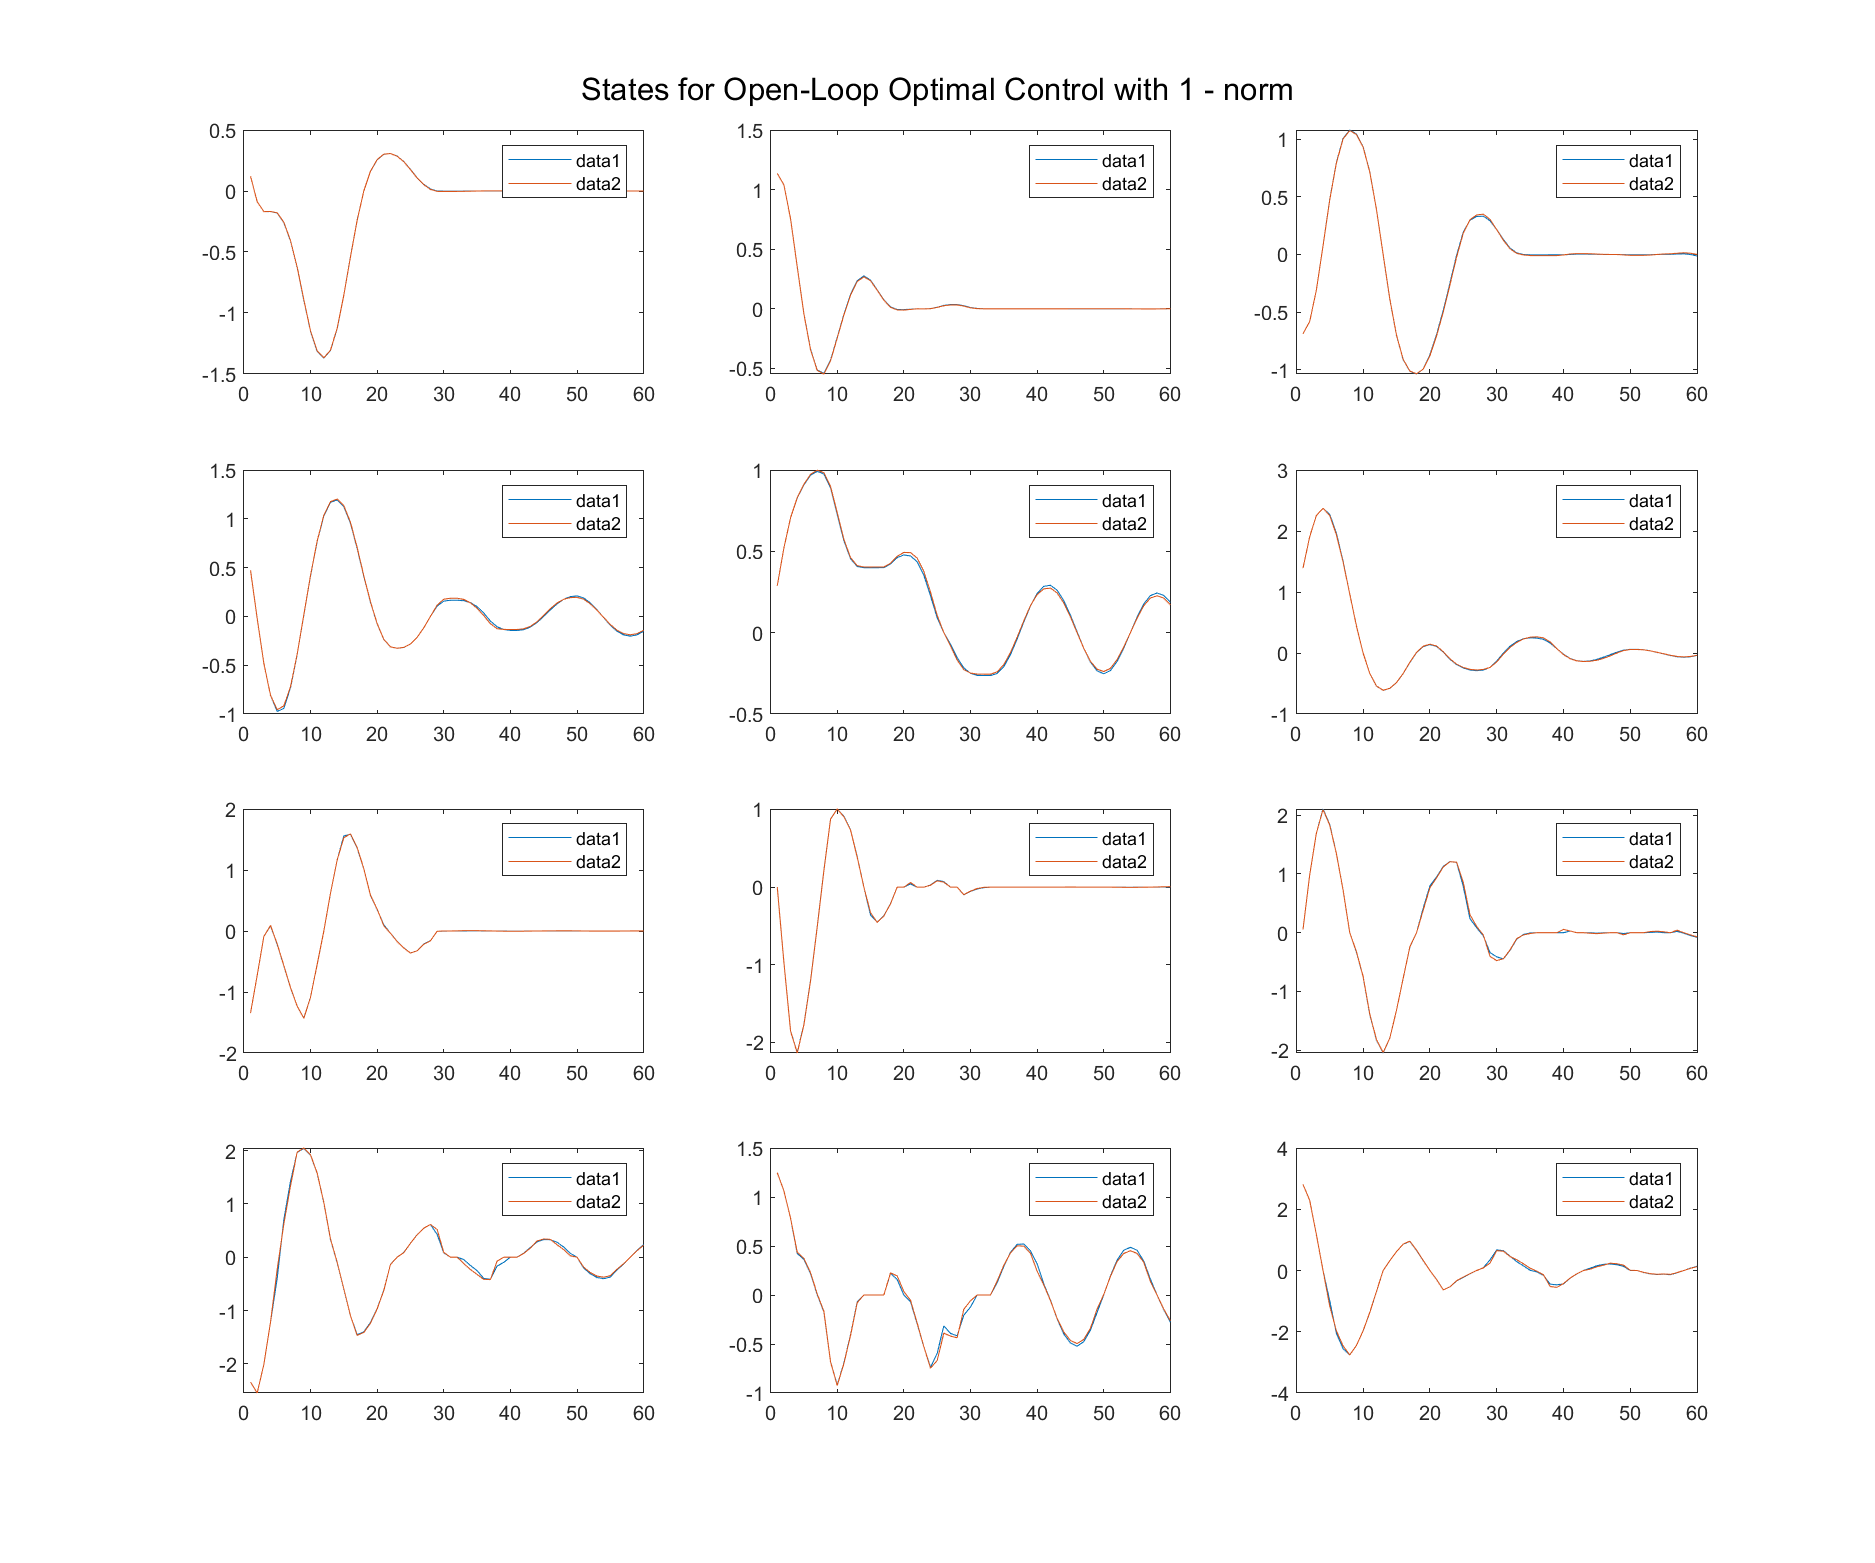
\includegraphics[width=1\linewidth]{fig/pblm1_1n_x}
	\caption{States for Open-loop control comparing methods for 1-norm.}
	\label{fig:pblm11nx}
\end{figure}\newpage

\begin{figure}[h]
	\centering
	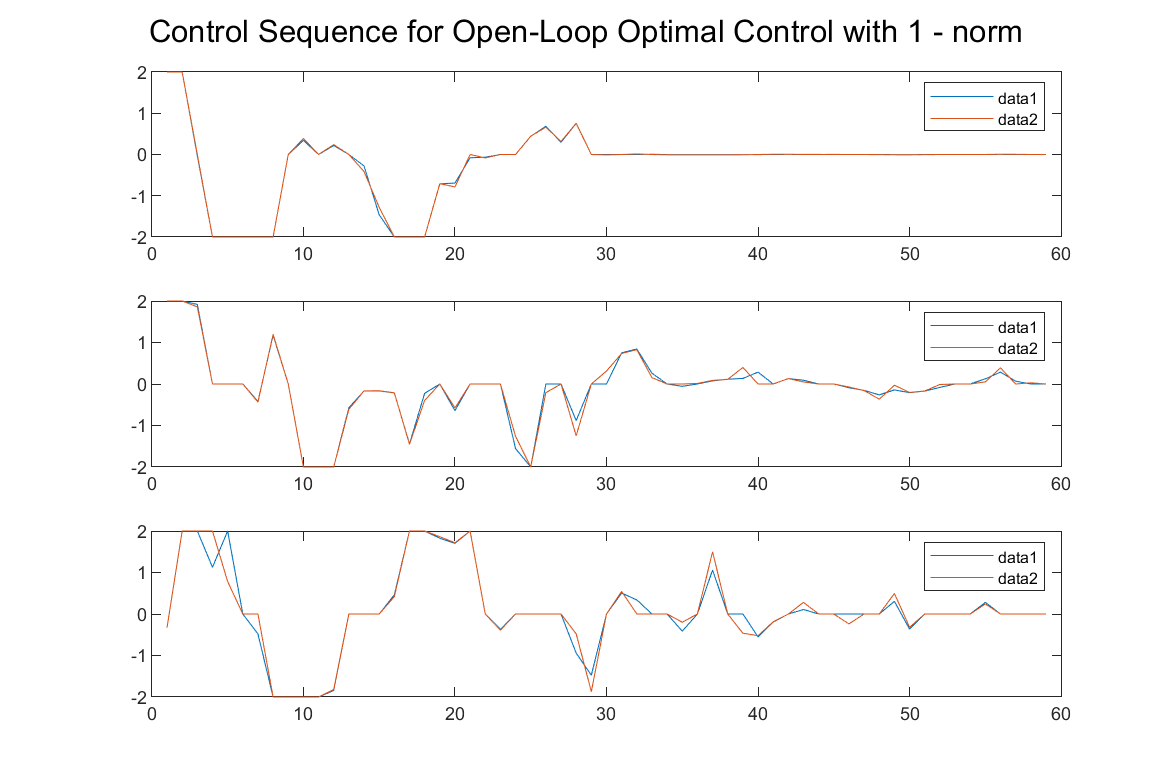
\includegraphics[width=1\linewidth]{fig/pblm1_1n_u}
	\caption{Inputs for Open-loop control comparing methods for 1-norm.}
	\label{fig:pblm11nu}
\end{figure}

\newpage
\section{Problem 2: Minimum time state transfer via quasiconvex optimization.}
Consider the LTI system:
\begin{equation}\label{eq:quasiconvex_opt_def}
	\begin{aligned}
		x_{t+1} &= Ax_t + B u_t, \ \forall t = 0,\dots,T\\
		\underline{u} &\leq u_t \leq \bar{u}, \ \forall t = 0,\dots,T
	\end{aligned}
\end{equation}
with $x_0$ as the initial state.\\

\textbf{Problem:}
Show that the minimum time required to transfer the system from $x_0$ to $x_{des}$, given as
\begin{equation}\label{eq:qualiconvex_problem_result}
	f(u_0,\dots,u_T) = \min \{\tau \ | \ x_t = x_{des} \ \text{for} \ \tau \leq t \leq {T+1}\}
\end{equation}
is a quasiconvex function of the control input sequence. Implement a bisection algorithm to solve the problem for the given data.\\

\textbf{Solution:}
It is evident from the definition of the minimization problem that the time required to reach the final state for each sequence of inputs is a convex optimization problem. From that, it is known that the function overall is a quasi-convex optimization problem defined as:
\optpblm{\tau}{
	x_{t+1} = Ax_t + B u_t \ \forall t = 0,\dots,T\\
	&\underline{u} \leq u_t \leq \bar{u} \ \forall t = 0,\dots,T\\
	&x(0) = x_0\\
	&x_t = x_{des} \ \forall t \in \{t \ | \ \tau \leq t \leq {T+1}\}
	}

For simplicity, we will be relaxing the final state to just reaching it at the earliest instead of remaining at rest:
$$x_\tau = x_{des}$$

A bisection algorithm can then be implemented to solve this as done using the MATLAB code shown in \appendixname \ \ref{apx:pblm2_matlab}. The result of this was a minimum value $$t = 51, \text{ or } \tau = 10.2$$

\newpage
The resulting system response and control sequence are provided as:
\begin{figure}[h]
	\centering
	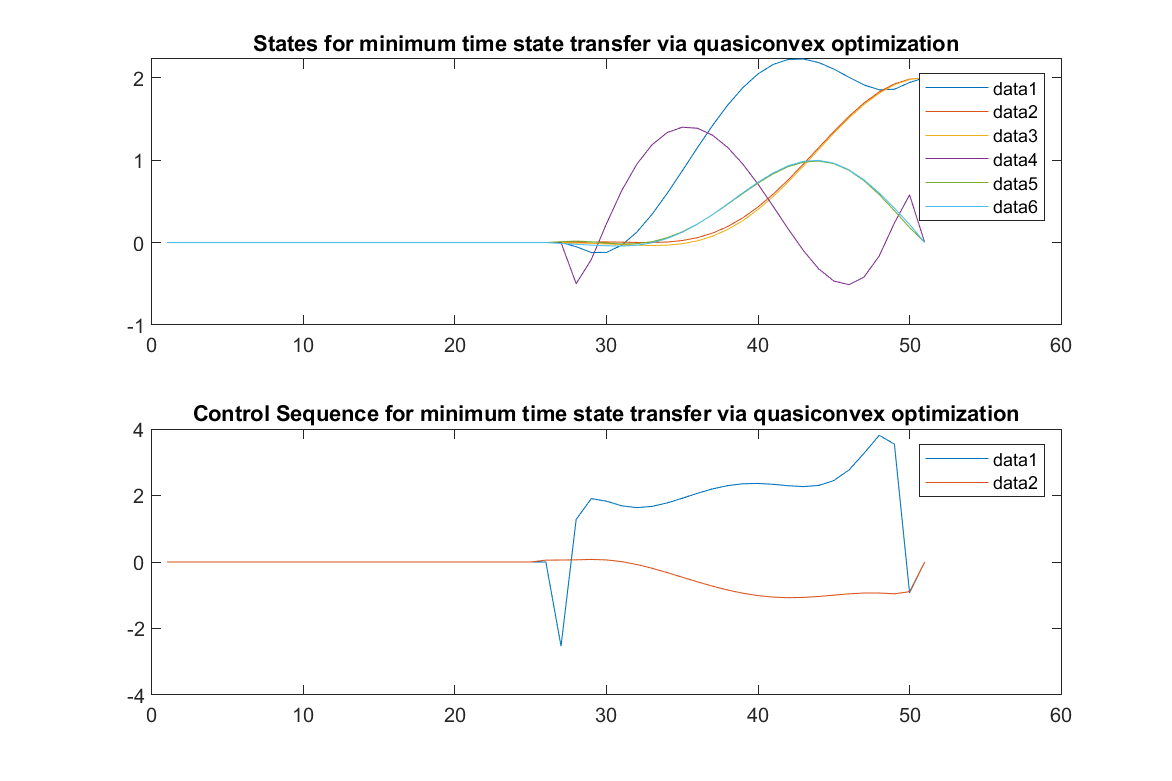
\includegraphics[width=1\linewidth]{fig/pblm2}
	\caption{Results for problem 2.}
	\label{fig:pblm2}
\end{figure}

\newpage
\section{Problem 3: State feedback control design via SDP}
Feedback control problems can be formulated using a semidefinite program, such as
\begin{equation}\label{eq:feedback_control_def}
	\begin{aligned}
		\text{maximize} \hspace{0.5in}& \trace \{P\}\\
		\text{subject to} \hspace{0.5in}
		& \mqty [R + B^T PB & B^T PA\\
				 A^T PB & Q + A^T P A - P] \succeq 0\\
				 & P \succeq 0
	\end{aligned}
\end{equation}
with variable $P \in S^n$ and problem data $A\in \real^{n\cross n}, B \in\real^{n\cross m}, Q \in S^n_+, \real \in S^m_{++}$.\\

This problem is equivalent to the solution to the optimal solution to the infinite-horizon LQR problem:
\begin{equation}\label{eq:LQR_control_def}
	\begin{aligned}
		\text{minimze} \hspace{0.5in}& \sum_{t=0}^\infty x_t^T Q x_t + u_t^T R u_t\\
		\text{subject to} \hspace{0.5in}
		& x_{t+1} = Ax_t + B u_t, \ t \geq 0, \ x(t=0) = x_0
	\end{aligned}
\end{equation}
This is also equivelent to the solution the the discrete-time richotte equation (DARE) and can be solved in matlab with dare(A,B,Q,R). The solution to the feedback controller is
\begin{equation}\label{eq:LQR_control_solution}
	u_t = K x_t\\
	K = -\qty(R + B^T B)^{-1} B^T P^* A
\end{equation}

\textbf{Problem:}
Confirm the solution to the SDP given in \eqref{eq:feedback_control_def} is equivalent to the LQR problem given in \eqref{eq:LQR_control_def} for multiple randomly generated problems.

\textbf{Solution:}
CVX in MATLAB was used and the code can be found in \appendixname \ref{apx:pblm3_matlab}.The full set of results are provided in \appendixname \ref{apx:pblm3_results} for various randomly generated problems and solutions. The following is a few of P equivelent reuslts.

\begin{Verbatim}
	P_cvx =
	
	20.3336   10.5025   -3.3125   37.1904
	10.5025   12.9464   -1.8618   32.8376
	-3.3125   -1.8618    2.3441   -4.8914
	37.1904   32.8376   -4.8914   97.6353
	
	
	P_dare =
	
	20.3336   10.5025   -3.3125   37.1904
	10.5025   12.9464   -1.8618   32.8376
	-3.3125   -1.8618    2.3441   -4.8914
	37.1904   32.8376   -4.8914   97.6353
\end{Verbatim}
\begin{Verbatim}
	P_cvx =
	
	9.2752    0.3867    1.2843   -2.9794
	0.3867    4.4079    0.6458    1.1789
	1.2843    0.6458    1.9253    0.5430
	-2.9794    1.1789    0.5430    4.4857
	
	
	P_dare =
	
	9.2752    0.3867    1.2843   -2.9794
	0.3867    4.4079    0.6458    1.1789
	1.2843    0.6458    1.9253    0.5430
	-2.9794    1.1789    0.5430    4.4857
\end{Verbatim}
\begin{Verbatim}
	P_cvx =
	
	101.8040  -50.0081   -0.8792  117.2149
	-50.0081   28.3481    2.3037  -57.6749
	-0.8792    2.3037    4.1602    0.2983
	117.2149  -57.6749    0.2983  136.1756
	
	
	P_dare =
	
	101.8040  -50.0081   -0.8792  117.2149
	-50.0081   28.3481    2.3037  -57.6749
	-0.8792    2.3037    4.1602    0.2983
	117.2149  -57.6749    0.2983  136.1756
\end{Verbatim}

\newpage
\appendix
\section{MATLAB Code:}\label{apx:matlab}
All code I write in this course can be found on my GitHub repository:\\
\href{https://github.com/jonaswagner2826/MECH6337}{https://github.com/jonaswagner2826/MECH6327}
\lstinputlisting[caption={MECH6327\_HW3},label={script:HW3}]{MECH6327_HW3.m}

\newpage
\section{Problem 3 MATLAB Code:}\label{apx:pblm1_matlab}
All code I write in this course can be found on my GitHub repository:\\
\href{https://github.com/jonaswagner2826/MECH6327}{https://github.com/jonaswagner2826/MECH6327}
% MECH6313_HW3_pblm1
\lstinputlisting[caption={MECH6327\_HW3\_pblm1},label={script:HW3}]{MECH6327_HW3_pblm1.m}

\newpage
\section{Problem 3 MATLAB Code:}\label{apx:pblm2_matlab}
All code I write in this course can be found on my GitHub repository:\\
\href{https://github.com/jonaswagner2826/MECH6327}{https://github.com/jonaswagner2826/MECH6327}
% MECH6313_HW3_pblm2
\lstinputlisting[caption={MECH6327\_HW3\_pblm2},label={script:HW3}]{MECH6327_HW3_pblm2.m}

\newpage
\section{Problem 3 MATLAB Code:}\label{apx:pblm3_matlab}
All code I write in this course can be found on my GitHub repository:\\
\href{https://github.com/jonaswagner2826/MECH6327}{https://github.com/jonaswagner2826/MECH6327}
% MECH6313_HW3_pblm3
\lstinputlisting[caption={MECH6327\_HW3\_pblm3},label={script:HW3}]{MECH6327_HW3_pblm3.m}

\newpage
\section{Problem 3 MATLAB Results:}\label{apx:pblm3_results}

\begin{Verbatim}
	>> MECH6327_HW3_pblm3
	
	A =
	
	1.1002   -1.1372    1.1077    0.2641
	0.1751    0.6430    0.8205    3.1585
	1.0036   -0.0128   -0.8176    1.2266
	1.5110    0.9143   -0.1265    2.3206
	
	
	B =
	
	0.4145    1.2416
	0.2118   -0.1576
	0.6132   -1.3736
	-0.5278    0.8708
	
	
	Q =
	
	0.4766    0.4525    0.2565    0.4911
	0.4525    0.5808    0.3777    0.7950
	0.2565    0.3777    0.4440    0.4396
	0.4911    0.7950    0.4396    1.2997
	
	
	R =
	
	1.1591    0.8154
	0.8154    0.7716
	
	
	Calling SDPT3 4.0: 31 variables, 10 equality constraints
	For improved efficiency, SDPT3 is solving the dual problem.
	------------------------------------------------------------
	
	num. of constraints = 10
	dim. of sdp    var  = 10,   num. of sdp  blk  =  2
	*******************************************************************
	SDPT3: Infeasible path-following algorithms
	*******************************************************************
	version  predcorr  gam  expon  scale_data
	HKM      1      0.000   1        0    
	it pstep dstep pinfeas dinfeas  gap      prim-obj      dual-obj    cputime
	-------------------------------------------------------------------
	0|0.000|0.000|8.4e+01|1.2e+01|1.5e+03| 4.731862e+01  0.000000e+00| 0:0:00| chol  1  1 
	1|0.894|0.821|8.9e+00|2.3e+00|2.2e+02| 2.141617e+01  1.453677e+01| 0:0:00| chol  1  1 
	2|0.833|0.841|1.5e+00|3.7e-01|5.1e+01| 2.431086e+01  1.330905e+01| 0:0:00| chol  1  1 
	3|0.515|0.846|7.2e-01|5.7e-02|2.1e+01| 2.140755e+01  2.132680e+01| 0:0:00| chol  1  1 
	4|0.187|0.237|5.9e-01|4.4e-02|1.9e+01| 2.434592e+01  7.419460e+01| 0:0:00| chol  1  1 
	5|0.061|0.042|5.5e-01|4.2e-02|2.7e+01| 3.321322e+01  1.216786e+02| 0:0:00| chol  1  1 
	6|0.104|0.026|4.9e-01|4.1e-02|5.4e+01| 6.400240e+01  6.740367e+01| 0:0:00| chol  1  1 
	7|0.129|0.433|4.3e-01|2.3e-02|5.0e+01| 7.772307e+01  1.153429e+02| 0:0:00| chol  1  1 
	8|1.000|0.825|1.4e-08|4.0e-03|4.5e+01| 1.616373e+02  1.181693e+02| 0:0:00| chol  1  1 
	9|0.962|0.980|2.6e-07|7.9e-05|1.8e+00| 1.344089e+02  1.326294e+02| 0:0:00| chol  1  1 
	10|0.965|0.977|9.4e-09|1.8e-06|5.8e-02| 1.333014e+02  1.332444e+02| 0:0:00| chol  1  1 
	11|0.958|1.000|3.9e-10|1.9e-09|3.6e-03| 1.332623e+02  1.332587e+02| 0:0:00| chol  1  1 
	12|0.987|1.000|7.9e-12|7.9e-11|2.8e-04| 1.332596e+02  1.332594e+02| 0:0:00| chol  1  1 
	13|0.952|0.987|1.2e-11|2.6e-12|1.3e-05| 1.332595e+02  1.332595e+02| 0:0:00| chol  1  1 
	14|1.000|1.000|5.2e-12|2.3e-12|1.2e-06| 1.332595e+02  1.332595e+02| 0:0:00|
	stop: max(relative gap, infeasibilities) < 1.49e-08
	-------------------------------------------------------------------
	number of iterations   = 14
	primal objective value =  1.33259457e+02
	dual   objective value =  1.33259456e+02
	gap := trace(XZ)       = 1.15e-06
	relative gap           = 4.31e-09
	actual relative gap    = 4.31e-09
	rel. primal infeas (scaled problem)   = 5.20e-12
	rel. dual     "        "       "      = 2.32e-12
	rel. primal infeas (unscaled problem) = 0.00e+00
	rel. dual     "        "       "      = 0.00e+00
	norm(X), norm(y), norm(Z) = 1.7e+02, 1.1e+02, 1.7e+03
	norm(A), norm(b), norm(C) = 3.5e+01, 3.0e+00, 3.9e+00
	Total CPU time (secs)  = 0.47  
	CPU time per iteration = 0.03  
	termination code       =  0
	DIMACS: 7.8e-12  0.0e+00  4.0e-12  0.0e+00  4.3e-09  4.3e-09
	-------------------------------------------------------------------
	
	------------------------------------------------------------
	Status: Solved
	Optimal value (cvx_optval): -133.259
	
	
	P_cvx =
	
	20.3336   10.5025   -3.3125   37.1904
	10.5025   12.9464   -1.8618   32.8376
	-3.3125   -1.8618    2.3441   -4.8914
	37.1904   32.8376   -4.8914   97.6353
	
	
	K_cvx =
	
	1.3793    2.0277   -0.1335    4.7523
	-1.0233    0.0284   -0.4975   -1.2125
	
	
	P_dare =
	
	20.3336   10.5025   -3.3125   37.1904
	10.5025   12.9464   -1.8618   32.8376
	-3.3125   -1.8618    2.3441   -4.8914
	37.1904   32.8376   -4.8914   97.6353
	
	
	K_dare =
	
	-1.3793   -2.0277    0.1335   -4.7523
	1.0233   -0.0284    0.4975    1.2125
	
	
	P_cvx =
	
	20.3336   10.5025   -3.3125   37.1904
	10.5025   12.9464   -1.8618   32.8376
	-3.3125   -1.8618    2.3441   -4.8914
	37.1904   32.8376   -4.8914   97.6353
	
	
	P_dare =
	
	20.3336   10.5025   -3.3125   37.1904
	10.5025   12.9464   -1.8618   32.8376
	-3.3125   -1.8618    2.3441   -4.8914
	37.1904   32.8376   -4.8914   97.6353
	
	>> MECH6327_HW3_pblm3
	
	A =
	
	-0.8568    1.3798   -0.6563    1.1284
	0.0484    0.0951   -0.1250    0.7425
	-0.6649   -0.4271   -0.5305    1.1436
	1.4527    0.5108    0.1056   -0.9147
	
	
	B =
	
	0.1798    1.2963
	-0.9833    1.0992
	0.3848    0.6532
	0.3257   -0.5051
	
	
	Q =
	
	0.3838    0.3714    0.4771    0.6771
	0.3714    1.2344    1.2453    1.0731
	0.4771    1.2453    1.4076    1.4208
	0.6771    1.0731    1.4208    2.1397
	
	
	R =
	
	0.5081    0.7407
	0.7407    1.1909
	
	
	Calling SDPT3 4.0: 31 variables, 10 equality constraints
	For improved efficiency, SDPT3 is solving the dual problem.
	------------------------------------------------------------
	
	num. of constraints = 10
	dim. of sdp    var  = 10,   num. of sdp  blk  =  2
	*******************************************************************
	SDPT3: Infeasible path-following algorithms
	*******************************************************************
	version  predcorr  gam  expon  scale_data
	HKM      1      0.000   1        0    
	it pstep dstep pinfeas dinfeas  gap      prim-obj      dual-obj    cputime
	-------------------------------------------------------------------
	0|0.000|0.000|4.4e+01|5.2e+00|1.0e+03| 6.864540e+01  0.000000e+00| 0:0:00| chol  1  1 
	1|0.886|0.852|5.0e+00|8.2e-01|1.7e+02| 5.707109e+01  1.265425e+01| 0:0:00| chol  1  1 
	2|0.782|1.000|1.1e+00|5.5e-03|5.2e+01| 5.048488e+01  1.175262e+01| 0:0:00| chol  1  1 
	3|0.752|1.000|2.7e-01|5.5e-04|1.6e+01| 2.602445e+01  1.535157e+01| 0:0:00| chol  1  1 
	4|1.000|0.756|1.8e-07|1.8e-04|7.3e+00| 2.578672e+01  1.846254e+01| 0:0:00| chol  1  1 
	5|0.933|1.000|1.8e-08|5.6e-06|5.8e-01| 2.048293e+01  1.990168e+01| 0:0:00| chol  1  1 
	6|0.964|0.970|2.0e-09|7.1e-07|2.9e-02| 2.011379e+01  2.008495e+01| 0:0:00| chol  1  1 
	7|0.965|1.000|6.3e-10|5.6e-08|1.7e-03| 2.009536e+01  2.009368e+01| 0:0:00| chol  1  1 
	8|0.994|1.000|1.8e-10|1.3e-10|1.2e-04| 2.009415e+01  2.009404e+01| 0:0:00| chol  1  1 
	9|0.953|0.987|6.7e-11|3.7e-11|5.3e-06| 2.009409e+01  2.009408e+01| 0:0:00| chol  1  1 
	10|1.000|1.000|6.7e-15|1.3e-11|1.2e-06| 2.009408e+01  2.009408e+01| 0:0:00| chol  1  1 
	11|1.000|1.000|1.7e-14|1.0e-12|1.3e-08| 2.009408e+01  2.009408e+01| 0:0:00|
	stop: max(relative gap, infeasibilities) < 1.49e-08
	-------------------------------------------------------------------
	number of iterations   = 11
	primal objective value =  2.00940824e+01
	dual   objective value =  2.00940824e+01
	gap := trace(XZ)       = 1.33e-08
	relative gap           = 3.22e-10
	actual relative gap    = 3.22e-10
	rel. primal infeas (scaled problem)   = 1.70e-14
	rel. dual     "        "       "      = 1.00e-12
	rel. primal infeas (unscaled problem) = 0.00e+00
	rel. dual     "        "       "      = 0.00e+00
	norm(X), norm(y), norm(Z) = 8.9e+00, 1.2e+01, 8.9e+01
	norm(A), norm(b), norm(C) = 1.8e+01, 3.0e+00, 5.7e+00
	Total CPU time (secs)  = 0.42  
	CPU time per iteration = 0.04  
	termination code       =  0
	DIMACS: 2.6e-14  0.0e+00  1.8e-12  0.0e+00  3.2e-10  3.2e-10
	-------------------------------------------------------------------
	
	------------------------------------------------------------
	Status: Solved
	Optimal value (cvx_optval): -20.0941
	
	
	P_cvx =
	
	9.2752    0.3867    1.2843   -2.9794
	0.3867    4.4079    0.6458    1.1789
	1.2843    0.6458    1.9253    0.5430
	-2.9794    1.1789    0.5430    4.4857
	
	
	K_cvx =
	
	0.5888   -0.3683    0.2601   -0.1295
	0.7294   -0.5856    0.4291   -0.9410
	
	
	P_dare =
	
	9.2752    0.3867    1.2843   -2.9794
	0.3867    4.4079    0.6458    1.1789
	1.2843    0.6458    1.9253    0.5430
	-2.9794    1.1789    0.5430    4.4857
	
	
	K_dare =
	
	-0.5888    0.3683   -0.2601    0.1295
	-0.7294    0.5856   -0.4291    0.9410
	
	
	P_cvx =
	
	9.2752    0.3867    1.2843   -2.9794
	0.3867    4.4079    0.6458    1.1789
	1.2843    0.6458    1.9253    0.5430
	-2.9794    1.1789    0.5430    4.4857
	
	
	P_dare =
	
	9.2752    0.3867    1.2843   -2.9794
	0.3867    4.4079    0.6458    1.1789
	1.2843    0.6458    1.9253    0.5430
	-2.9794    1.1789    0.5430    4.4857
	
	>> MECH6327_HW3_pblm3
	
	A =
	
	-1.5312    0.7880    1.6345   -0.9443
	0.5046    0.2982   -0.6235   -0.6712
	-0.8642   -0.1637   -1.3501    0.5767
	-0.3766    0.6067   -1.1622   -2.0858
	
	
	B =
	
	0.2360    0.0076
	-0.7784   -0.9376
	1.0996   -0.6816
	-0.8556   -0.2601
	
	
	Q =
	
	1.5071    1.3058    1.2427    1.5227
	1.3058    2.0018    1.1626    1.6402
	1.2427    1.1626    1.9380    2.0005
	1.5227    1.6402    2.0005    2.2226
	
	
	R =
	
	0.1582    0.2334
	0.2334    0.4393
	
	
	Calling SDPT3 4.0: 31 variables, 10 equality constraints
	For improved efficiency, SDPT3 is solving the dual problem.
	------------------------------------------------------------
	
	num. of constraints = 10
	dim. of sdp    var  = 10,   num. of sdp  blk  =  2
	*******************************************************************
	SDPT3: Infeasible path-following algorithms
	*******************************************************************
	version  predcorr  gam  expon  scale_data
	HKM      1      0.000   1        0    
	it pstep dstep pinfeas dinfeas  gap      prim-obj      dual-obj    cputime
	-------------------------------------------------------------------
	0|0.000|0.000|4.4e+01|3.9e+00|1.0e+03| 8.266937e+01  0.000000e+00| 0:0:00| chol  1  1 
	1|0.818|0.880|8.1e+00|5.1e-01|1.7e+02| 3.173665e+01  9.183288e+00| 0:0:00| chol  1  1 
	2|0.761|0.758|1.9e+00|1.3e-01|6.0e+01| 2.745402e+01  1.125760e+01| 0:0:00| chol  1  1 
	3|0.553|0.897|8.6e-01|1.3e-02|2.5e+01| 2.195296e+01  1.974743e+01| 0:0:00| chol  1  1 
	4|0.169|0.214|7.2e-01|1.1e-02|2.1e+01| 2.472518e+01  1.029151e+02| 0:0:00| chol  1  1 
	5|0.017|0.022|7.1e-01|1.0e-02|3.3e+01| 3.109723e+01  1.695860e+02| 0:0:00| chol  1  1 
	6|0.061|0.035|6.6e-01|1.0e-02|7.8e+01| 8.019566e+01  2.054055e+02| 0:0:00| chol  1  1 
	7|0.423|0.391|3.8e-01|6.1e-03|1.4e+02| 2.228571e+02  2.222143e+02| 0:0:00| chol  1  1 
	8|1.000|0.531|8.3e-06|2.8e-03|1.1e+02| 3.445733e+02  2.448139e+02| 0:0:00| chol  2  1 
	9|0.952|1.000|1.7e-06|1.7e-06|1.6e+01| 2.823759e+02  2.660703e+02| 0:0:00| chol  1  1 
	10|0.950|0.991|8.3e-08|3.5e-07|1.1e+00| 2.712737e+02  2.701719e+02| 0:0:00| chol  1  1 
	11|1.000|1.000|2.1e-10|1.7e-08|1.1e-01| 2.705570e+02  2.704431e+02| 0:0:00| chol  1  1 
	12|0.959|0.980|1.7e-10|4.8e-10|4.0e-03| 2.704909e+02  2.704869e+02| 0:0:00| chol  1  1 
	13|0.993|1.000|1.0e-10|3.4e-11|2.4e-04| 2.704880e+02  2.704878e+02| 0:0:00| chol  1  1 
	14|0.954|0.989|8.0e-11|2.1e-11|1.1e-05| 2.704879e+02  2.704879e+02| 0:0:00| chol  1  1 
	15|1.000|1.000|1.7e-10|1.6e-11|1.0e-06| 2.704879e+02  2.704879e+02| 0:0:00|
	stop: max(relative gap, infeasibilities) < 1.49e-08
	-------------------------------------------------------------------
	number of iterations   = 15
	primal objective value =  2.70487886e+02
	dual   objective value =  2.70487885e+02
	gap := trace(XZ)       = 1.04e-06
	relative gap           = 1.92e-09
	actual relative gap    = 1.87e-09
	rel. primal infeas (scaled problem)   = 1.72e-10
	rel. dual     "        "       "      = 1.59e-11
	rel. primal infeas (unscaled problem) = 0.00e+00
	rel. dual     "        "       "      = 0.00e+00
	norm(X), norm(y), norm(Z) = 8.9e+02, 2.2e+02, 1.4e+03
	norm(A), norm(b), norm(C) = 2.2e+01, 3.0e+00, 7.5e+00
	Total CPU time (secs)  = 0.45  
	CPU time per iteration = 0.03  
	termination code       =  0
	DIMACS: 2.6e-10  0.0e+00  3.7e-11  0.0e+00  1.9e-09  1.9e-09
	-------------------------------------------------------------------
	
	------------------------------------------------------------
	Status: Solved
	Optimal value (cvx_optval): -270.488
	
	
	P_cvx =
	
	101.8040  -50.0081   -0.8792  117.2149
	-50.0081   28.3481    2.3037  -57.6749
	-0.8792    2.3037    4.1602    0.2983
	117.2149  -57.6749    0.2983  136.1756
	
	
	K_cvx =
	
	-4.7337    3.0098    1.0219   -6.7728
	0.2527   -0.0799   -1.2428    0.2020
	
	
	P_dare =
	
	101.8040  -50.0081   -0.8792  117.2149
	-50.0081   28.3481    2.3037  -57.6749
	-0.8792    2.3037    4.1602    0.2983
	117.2149  -57.6749    0.2983  136.1756
	
	
	K_dare =
	
	4.7337   -3.0098   -1.0219    6.7728
	-0.2527    0.0799    1.2428   -0.2020
	
	
	P_cvx =
	
	101.8040  -50.0081   -0.8792  117.2149
	-50.0081   28.3481    2.3037  -57.6749
	-0.8792    2.3037    4.1602    0.2983
	117.2149  -57.6749    0.2983  136.1756
	
	
	P_dare =
	
	101.8040  -50.0081   -0.8792  117.2149
	-50.0081   28.3481    2.3037  -57.6749
	-0.8792    2.3037    4.1602    0.2983
	117.2149  -57.6749    0.2983  136.1756
\end{Verbatim}



%\newpage
%\section*{}
%\bibliographystyle{ieeetr}
%\bibliography{mybib.bib}


\end{document}
